\documentclass[12pt]{article}

\usepackage{hyperref}
\usepackage{fullpage}
\usepackage{nopageno}
\usepackage{amsthm}
\usepackage{amsmath}
\usepackage{amssymb}
\newcommand{\R}{\mathbb{R}}
\newcommand{\N}{\mathbb{N}}
\usepackage[margin=1.5in]{geometry}
\usepackage{wasysym}
\usepackage{add-copyright}

\usepackage{graphicx}

\title{Homework 8}
\date{Due Wednesday, October 29, 2008}

\long\def\symbolfootnote[#1]#2{\begingroup%
\def\thefootnote{\fnsymbol{footnote}}\footnote[#1]{#2}\endgroup}

\begin{document}
\maketitle

\begin{description}

\item[(a)] Using blocks that are each $1$ inch wide, I build the
  following structure:
\begin{center}
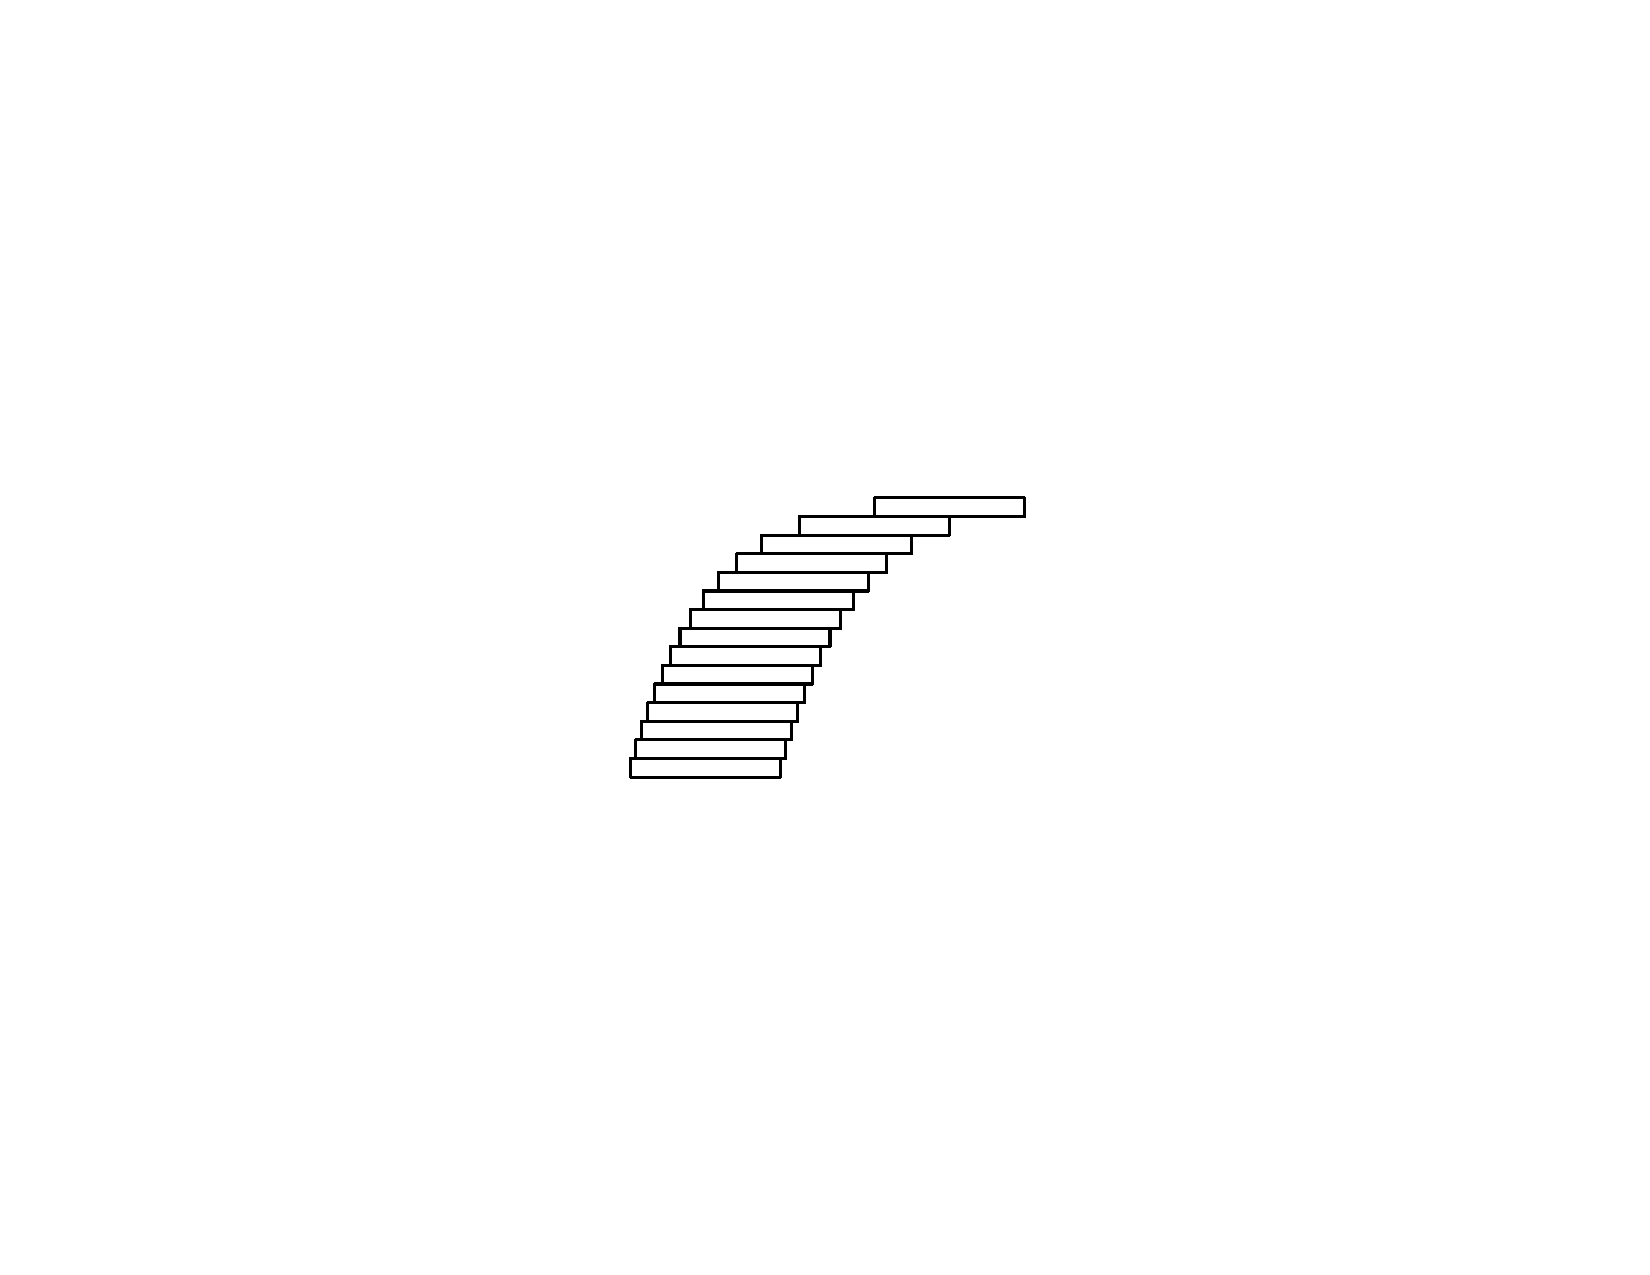
\includegraphics{blocks.pdf}
\end{center}
\noindent
The rightmost block is $1/2$ inch to the right of the block under it;
the second block from the top is $1/4$ inch to the right of the block
underneath it, the third block from the top is $1/6$ inch to the right
of the block under it.  In general, the $n^{\mbox{\underline{th}}}$
block from the top is $1/(2n)$ inches to the right of the
$(n+1)^{\mbox{\underline{th}}}$ block.
\begin{description}
\item[Part (i)] Prove that this structure will not fall over, no
matter how many blocks are used.
\item[Part (ii)] By using as many blocks as I like, how far to the
  right of the bottom block can I make the top block?
\end{description}

\vfill

\item[(b)] On page 592, in section 12.3, do problems: 1, 6, 8, 10, 18, 24, 31, 35.

\vfill

\end{description}


\end{document}
